\section{Multi-GPU Support}
\label{multi-GPU}
In this section, we characterize the performance of AlexNet built by different deep learning frameworks on multiple GPUs. AlexNet is trained on each framework with one, two, and four GPUs in this experiment. We exploits the data parallelism (explained in Section~\ref{sec:multiGPU-parallelism}) already available in the frameworks. Since Theano does not support mutiple GPUs, we compare only Caffe, CNTK, TensorFlow, and Torch. To train AlexNet, we select the fastest option based on the characteristics on a single GPU in Section~\ref{sec:singlGPU}

To exploit data parallelism, a GPU (say $GPU_0$) gathers intermediate gradient values to update network parameters stored in other GPUs ($GPU_1$, $GPU_2$, and $GPU_3$, assuming four GPUs). If gradients are gathered sequentially going through each GPU, the number of communications for gradient transfer between $GPU_0$ and other GPUs is $O(N-1)$, where $N$ is the number of GPUs. However, if gradients are gathered \Comment{with the parallel reduction algorithm}\cite{harris2007optimizing}, it is $O(\log{N})$ under the assumption that data trasfers can be parallelized if the source and destination GPUs are distinct. As long as a different GPU uses a different set of PCI-E lanes, the PCI-E bus has such property. Thus, our system supports the parallel reduction algorithm.

Ideally, the training time of AlexNet is expected to be reduced to $\frac{1}{N}$ if $N$ GPUs are used. However, this is not true because of the data trasfer caused by the gradient data exchange.
Since the size of gradient data in our AlexNet is about 250MB, the gradient transfer between two GPUs takes about 45ms. This is not negligible considering that one forward and backward computation takes  about 200ms with a batch size of 256.

\begin{figure*}[htbp]
  \centering
  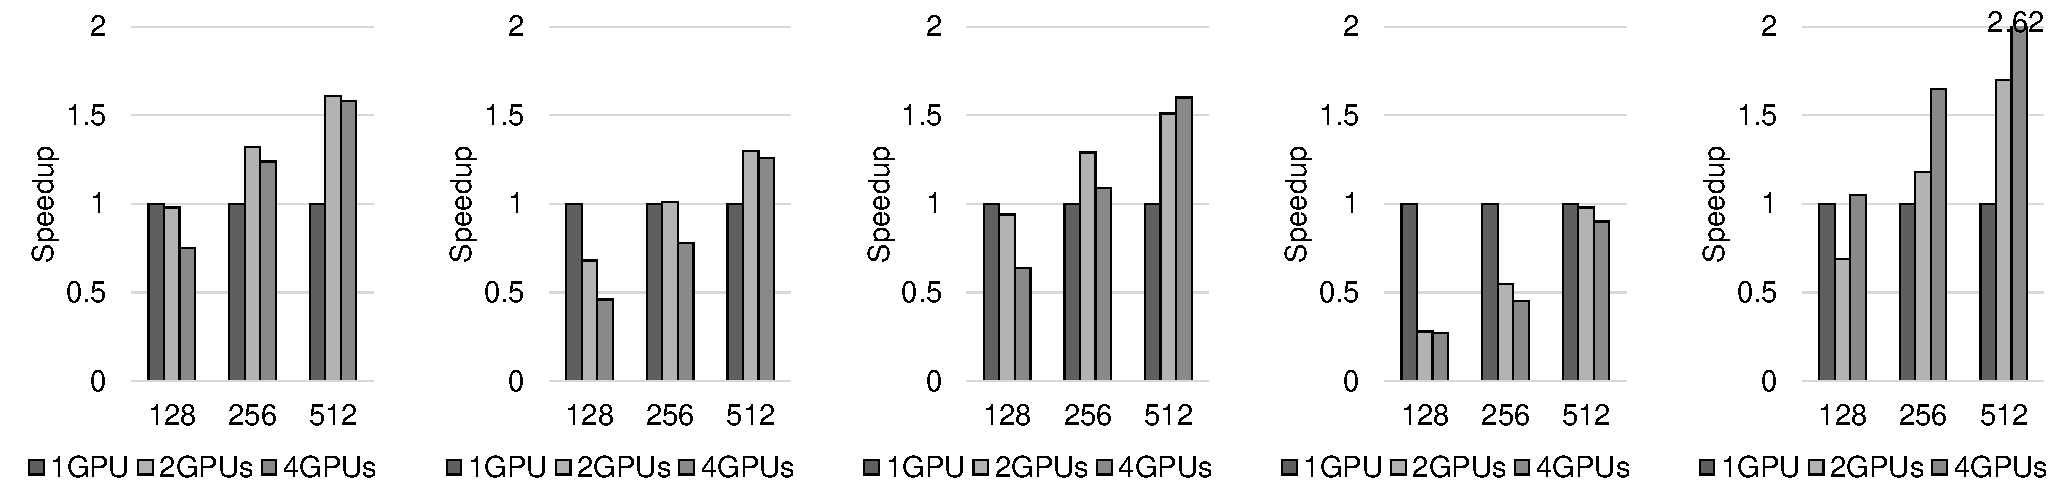
\includegraphics[width=.9\linewidth]{./figures/MG}
\caption{Speedup (over a single GPU) of multi-GPU training of AlexNet built by each framework.}
\label{fig_mg}
\end{figure*}

Figure~\ref{fig_mg} shows speedup obtained by multi-GPU training of our AlexNet built by each framework with different batch sizes and numbers of GPUs. We see that a bigger batch size makes the speedup higher. A batch size of 128 makes Caffe and Torch on two or four GPUs much slower than on a single GPU. A bigger batch size makes the computation time in each GPU longer. However, the number and size of data transfer is fixed because the number of network parameters remains the same. Thus, it is beneficial to use a bigger batch size.

We also see that the scalability of each framework is quite poor. The speedup of using four GPUs is slower than or comparable to that of using two GPUs for all frameworks. \Comment{The reason is, gradient transfer when using four GPUs still takes twice longer than using two GPUs, even though we use the $O(log N)$ algorithm to transfer data between GPUs.}

Torch and TensorFlow have comparable execution time on a single GPU. However, TensorFlow achieves higher speedup than Torch. Since TensorFlow handles gradients of each layer as an individual tensor, the gradients of each layer are transfered as soon as the backward computation of that layer finishes. On the other hand, Torch (and Caffe) references gradients of the entire network as a whole. Thus, it starts data transfer after all backward computations finish. That is, TensorFlow has more data transfer and computation overlapping.

\Comment{CNTK is special in terms of its multi-GPU support. Intermediate gradient values are gathered in the host memory, instead of the parallel reduction algorithm. Although data transfers can be parallelized, gradients are summed up by CPU and it takes much longer than computation time in GPUs. Thus, using any number of GPUs is slower than single GPU training.}

\Comment{Instead of using better reduction, they developed 1bit-SGD\cite{1-bit-stochastic-gradient-descent-and-application-to-data-parallel-distributed-training-of-speech-dnns}. In 1bit-SGD, only one bit per gradient is transfered, reducing memory transfers and CPU computation by a factor of 32 compared to when using the single-precision FP format. This greatly improves scalability to almost linear scale, at the cost of slow convergence.}

\subsection{Summary}

\Comment{We observed that current multi-GPU scalability of frameworks is bad and has many possibilities to be improved. TensorFlow-like data transfer and computation overlapping will be helpful to improve the performance of the framework on a multi-GPU context. Reducing the size of gradients by using approximating the exact value with less accuracy (\textit{e.g.}, using the half-precision FP format or only 1-bit like CNTK) will also improve scalability a lot. Reducing the number of gradients by resizing the CNN model and pruning will also work, especially in fully-connected layers because they contain more than 90\% of network parameters.}
